% !TeX program = pdflatex
% WCNC conference version (IEEE two-column conference template).
% Source: journal version main_lora_clean.tex (Computer Networks), condensed to the
% IEEE WCNC initial-submission limit of 6 printed pages, 10pt.
\documentclass[conference]{IEEEtran}
\IEEEoverridecommandlockouts
\usepackage{amsmath,amssymb,amsthm}
\usepackage{booktabs,multirow}
\usepackage{graphicx}
\usepackage{cite}
\usepackage{algorithm}
\usepackage{algorithmic}
\usepackage{tikz}
\usetikzlibrary{arrows.meta,positioning,fit,calc}
\usepackage[caption=false,font=footnotesize]{subfig}
\newtheorem{proposition}{Proposition}
\emergencystretch=1.5em

\begin{document}
\linespread{0.96}\selectfont

\title{Deadline-Aware Adaptive-Rank Federated LoRA over Mobile Edge Networks}

\author{\IEEEauthorblockN{Wenyu Ma, Tao Hu\IEEEauthorrefmark{1}, Xinlei Liu}
\IEEEauthorblockA{Information Engineering University, Zhengzhou 450001, China\\
Key Laboratory of Cyberspace Endogenous Safety and Security of Henan Province\\
Key Laboratory of Cyberspace Security, Ministry of Education of China\\
\IEEEauthorrefmark{1}Corresponding author: hutaondsc@163.com}}

\maketitle

\begin{abstract}
Federated LoRA reduces model-update traffic, but a fixed adaptation rank is poorly matched to time-varying mobile edge links. A high-rank update may miss a round deadline, while a uniformly low rank underuses a stable link. We therefore treat the LoRA rank as a network-visible resource. Each round is formulated as a joint client--rank assignment that maximizes expected useful updates under communication and participation constraints. The scheduler couples a mobility-conditioned timely-delivery probability with a saturating adaptation-capacity gain. A pseudo-polynomial dynamic program then solves this estimated, discretized per-round problem optimally on its budget grid. A rank-masked average over a frozen factor supports heterogeneous client ranks. Experiments combine a real federated LoRA trainer on three non-IID datasets with a 500-client scheduling simulator. The trainer also runs a joint client--rank DP arm. Under a 0.25\,s deadline, adaptive ranking achieves accuracy comparable to fixed rank 16 while reducing update bytes by 14\%. Volume-aligned full-parameter updates use $2.2\times$ the bytes and deliver only 4\% on time. In binding regimes, the dynamic program improves expected useful updates by up to 10\% over greedy scheduling and runs in 33--836\,ms for 500 clients.
\end{abstract}

\begin{IEEEkeywords}
federated learning, low-rank adaptation, mobile edge computing, deadline scheduling, resource allocation
\end{IEEEkeywords}

\section{Introduction}
\label{sec:intro}

Mobile edge networks increasingly host federated learning (FL) workloads in which heterogeneous clients such as smartphones, vehicles, UAVs, and satellite terminals collaborate on a shared model without exposing raw data \cite{mcmahan2017fedavg,liu2018sagin,mahboob2024ntn}. The dominant cost is the uplink: full-parameter updates saturate wireless capacity and frequently miss round deadlines when links degrade during handover or outage \cite{razmi2022ground,tang2023flsagin,qin2024dfrl,ribero2023intermittent}. Low-rank adaptation (LoRA) has therefore become an attractive transmission format for FL, because only two small factor matrices per adapted layer are communicated instead of the full weight delta \cite{hu2022lora,babakniya2023slora,zhang2024fedit}.

Existing Federated LoRA systems usually treat the rank $r$ as a fixed model hyperparameter shared by all clients and rounds. This treatment overlooks a network-visible scheduling dimension. The rank determines the number of transmitted parameters and therefore affects transmission time. A larger rank can increase the probability of missing the deadline on a time-varying link. A smaller rank can underuse a stable link. \emph{The LoRA rank is thus a network scheduling variable}, as well as a learning parameter. Selecting the rank for each client and round turns link heterogeneity into a controllable trade-off between adaptation capacity and timely delivery.

This paper makes three contributions:
\begin{itemize}
\item \textbf{Joint client--rank scheduling.} We link rank-dependent update size to processing and transmission time, mobility-conditioned timely-delivery probability $P_{\mathrm{on}}(r)$, and saturating adaptation gain $G(r)$. The resulting multiple-choice knapsack maximizes expected useful updates; a pseudo-polynomial dynamic program is optimal for the budget-discretized, estimated per-round problem (Sections~\ref{sec:model}--\ref{sec:solver}).
\item \textbf{Heterogeneous-rank aggregation.} We combine rank masking with a shared frozen factor. Under the same frozen $A$ and shared coordinates, averaging the factor equals averaging the update, and low-rank clients cannot dilute coordinates used only by higher-rank clients. This mechanism supports heterogeneous ranks; it is not a general rule for jointly trained factors (Section~\ref{sec:aggregation}).
\item \textbf{End-to-end evaluation.} The trainer compares a fair-cohort rank rule against the full joint client--rank DP arm on three non-IID datasets, and a 500-client simulator scales the joint scheduler. Together they show accuracy parity among the evaluated ranks, 14\% fewer bytes than fixed rank 16 under deadline stress, and up to 10\% more expected useful updates than greedy scheduling in binding regimes (Section~\ref{sec:eval}).
\end{itemize}

A preliminary poster considered client--protection scheduling in space--air--ground networks \cite{ma2026mswim}. The present work studies a different decision variable, solver, and evaluation setting. We report learning and network metrics separately. The expected benefit of rank adaptation is improved delivery efficiency, rather than universal accuracy gains.

\section{Related Work}
\label{sec:related}

\textbf{Parameter-efficient and federated LoRA.} LoRA freezes a pretrained backbone and learns $\Delta W = BA$ \cite{hu2022lora}. Federated variants then address how such adapters are shared. SLoRA averages sparse updates \cite{babakniya2023slora}, FedIT tunes instructions \cite{zhang2024fedit}, and FLoRA stacks aligned factors for heterogeneous ranks \cite{wang2024flora}. FFA-LoRA freezes the $A$ factor at its random initialization for stability in privacy-preserving fine-tuning \cite{sun2024ffalora}. On the scheduling side, SA-FedLoRA anneals the rank over rounds oblivious to network state \cite{yang2024safedlora}, and FedSA-LoRA aggregates only $A$ \cite{guo2025fedsalora}. These works mainly optimize learning-side objectives such as aggregation quality or adaptation schedules. They do not couple the per-round rank with link state and deadline, which is the gap this paper addresses.

\textbf{Communication-efficient FL and client selection.} Sparsification, quantization, and over-the-air aggregation compress a \emph{given} update \cite{oh2023fedqcs}; recent WCNC studies further use learned quantization and hierarchical model pruning to adapt wireless FL traffic \cite{zheng2023wcncquant,liu2024wcncpruning}. We instead choose the update structure, that is, its rank, before compression. This couples the decision to transmission time and deadline feasibility. Client selection admits useful clients under data, latency, and energy heterogeneity \cite{oort2021oort}. Related work addresses non-IID discrepancy, personalized model selection, and cache-limited online FL \cite{shen2023wcncnoniid,chen2024wcncmodel,hu2025wcnconline}, while deadline- and reliability-aware participation has been studied for mobile and non-terrestrial networks \cite{tang2023flsagin,qin2024dfrl,ribero2023intermittent}. These methods select clients or model operations but do not jointly choose each participant and its rank from link state; our paired decision $(i,r)$ yields a multiple-choice knapsack rather than a top-$K$ selection.

\section{System Model}
\label{sec:model}

\subsection{Mobile edge FL architecture}
An edge aggregator serves a client set $\mathcal{D}=\mathcal{D}_g\cup\mathcal{D}_a\cup\mathcal{D}_s$ of ground, aerial/UAV, and satellite-connected clients, as Fig.~\ref{fig:system} shows. Ground links are comparatively stable, aerial links face frequent handover, and satellite links suffer long propagation delay, intermittent visibility, and outages \cite{mahboob2024ntn,razmi2022ground}.

\begin{figure}[!t]
	\centering
	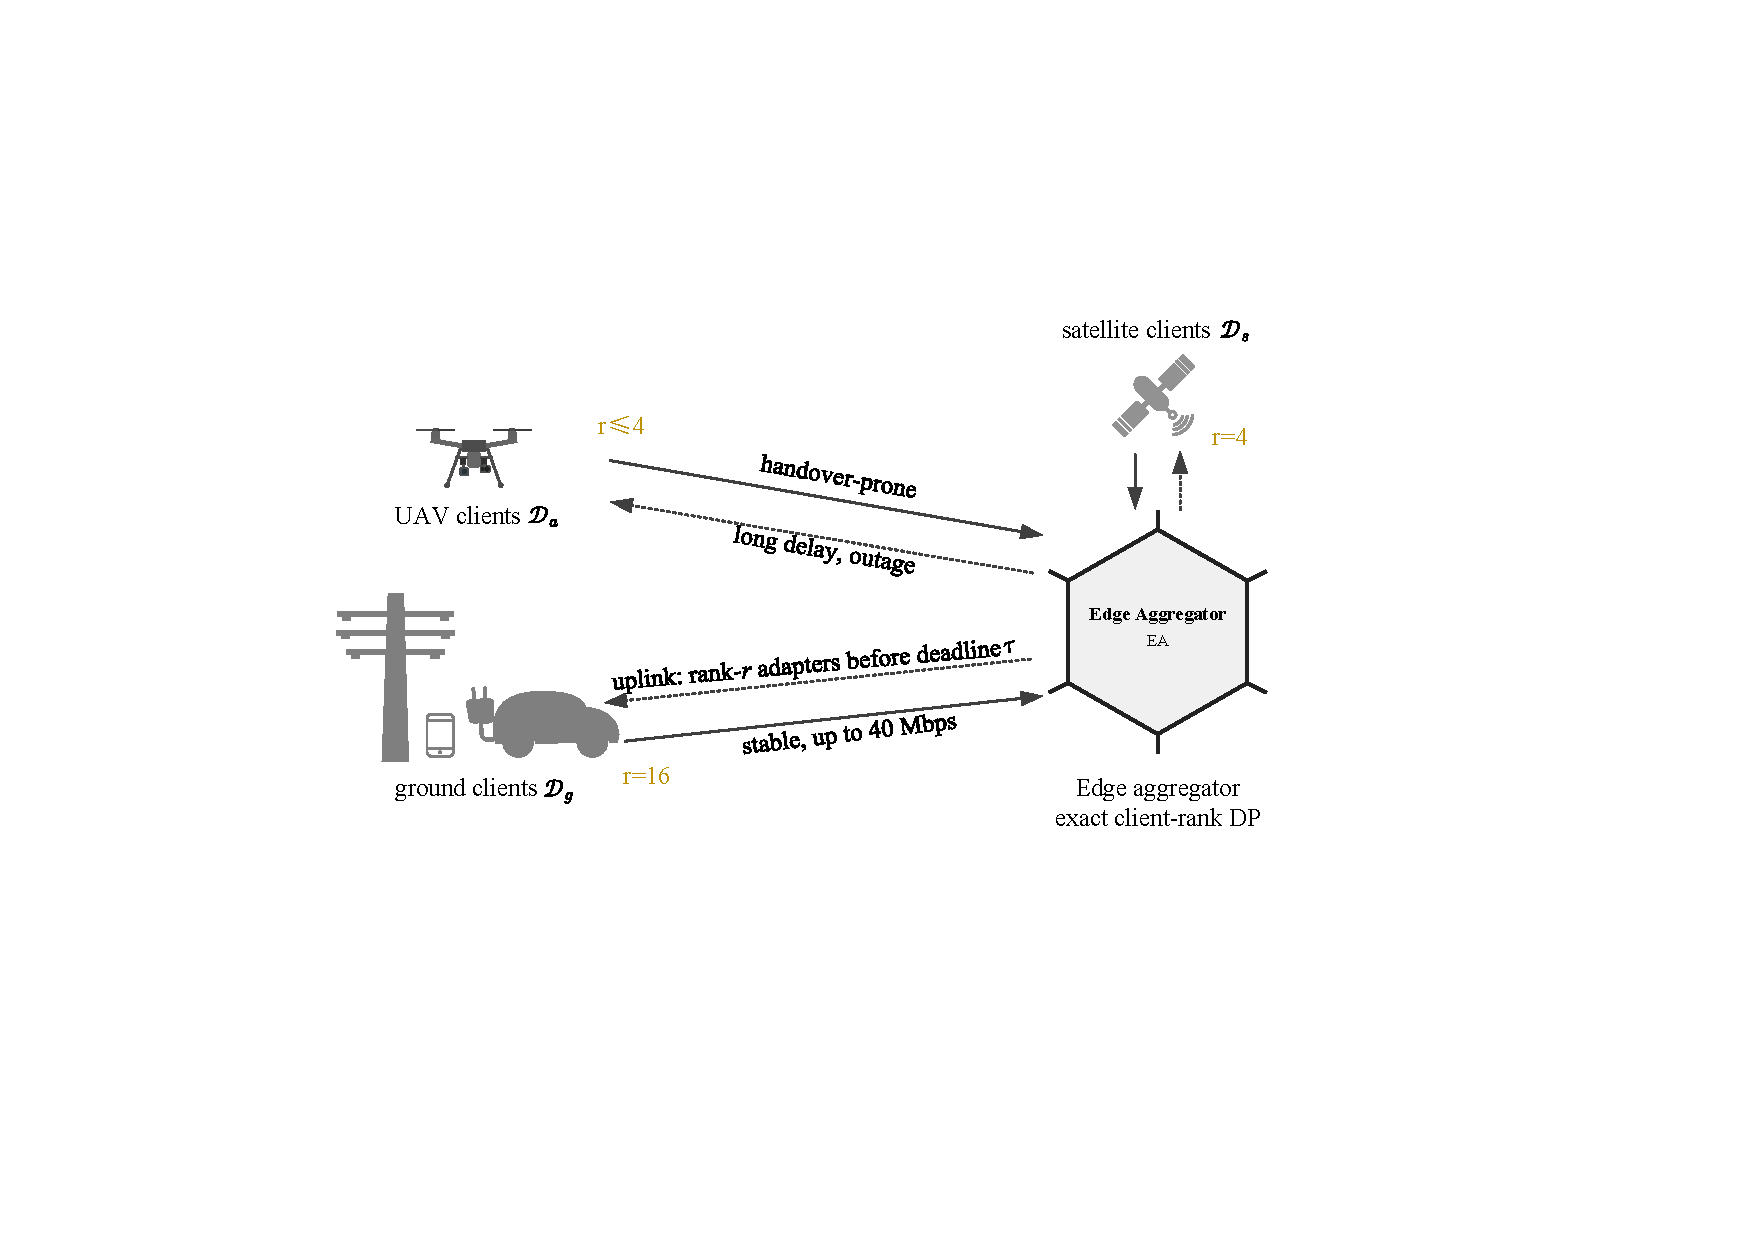
\includegraphics[width=0.9\linewidth]{wcnc.pdf}
	\vspace{-0.6em}
	\caption{System architecture: ground, aerial, and satellite clients federate LoRA adapters around an edge aggregator. Uplink carries rank-$r$ adapters before deadline $\tau$; downlink broadcasts $w^t$; heterogeneous updates are aggregated by rank-masked averaging over a frozen factor.}
	\label{fig:system}
\end{figure}


\subsection{Federated LoRA rounds}
Let $w^t$ be the frozen backbone broadcast at round $t$. Client $i$ trains LoRA factors $B_{i,\ell}\in\mathbb R^{d_\ell\times r_{\max}}$ and $A_{i,\ell}\in\mathbb R^{r_{\max}\times k_\ell}$ for adapted layers $\ell\in\mathcal L$ of input--output dimension $d_\ell\times k_\ell$; scheduling at rank $r$ keeps only the first $r$ columns of $B_{i,\ell}$ and rows of $A_{i,\ell}$, so $\Delta W_{i,\ell}=B_{i,\ell}A_{i,\ell}$ has rank $\le r$. Each round then proceeds in order. The aggregator broadcasts the backbone and adapter state and observes client link states. It solves the client--rank assignment under deadline, budget, and participation constraints. Admitted clients train locally and upload rank-$r$ adapters within the upload window $\tau$. Timely updates are then aggregated with data-size weights, and late or lost updates are discarded because stale updates slow convergence.

\subsection{Link, mobility, and delivery model}
At decision time each client exposes an observable state $x_i^t$. This state contains the estimated uplink rate $\bar R_i^t$ (Mbps), propagation delay $d_i^t$, loss probability $p_i^t$, and mobility features such as serving node, velocity, and link trend. The realized rate $R_i^t$, handover event $H_i^t\in\{0,1\}$, and loss indicator $J_i^t$ are unknown at decision time. For an update of $B_i^t(r)$ megabytes,
\begin{equation}
T_i^t(r)=T_{\rm train,i}(r)+T_{\rm proc,i}(r)+\frac{8\,B_i^t(r)}{R_i^t}+d_i^t+H_i^t\Delta d_h,
\label{eq:delivery}
\end{equation}
where $\Delta d_h$ is the handover penalty and $T_{\rm train},T_{\rm proc}$ grow weakly with $r$. The factor 8 converts megabytes to megabits for an Mbps link. Timely delivery is the joint event
\begin{equation}
P_{\rm on,i}^t(r)=\Pr\!\left(T_i^t(r)\le\tau,\;J_i^t=0\mid x_i^t\right),
\label{eq:pon}
\end{equation}
The probability is estimated before the update is transmitted, so no future outcome is used in the decision. Equation \eqref{eq:delivery} is the physical process model. The scheduler instead uses a simplified hazard-form estimator
\begin{equation}
\hat P_{\rm on,i}^t(r)=\exp\!\big(-\mu_i^t\big)\exp\!\Big(-\frac{8\,B_i^t(r)}{\bar R_i^t\,\tau}\Big),
\label{eq:hazard}
\end{equation}
where $\mu_i^t$ is the client's mobility intensity for the round; in the prototype it is an experimental proxy that absorbs the loss, handover, and outage factors. In deployment, $\mu_i^t$ can be learned from observed outcomes, for example with an EWMA of failure events.

\subsection{Rank-dependent size and capacity}
With $\beta$ bits per parameter and $d_\ell,k_\ell$ in millions, the payload of a rank-$r$ update is
\begin{equation}
B_i^t(r)=\frac{\beta}{8}\;r\!\sum_{\ell\in\mathcal L}\big(d_\ell+k_\ell\big)+B_{\rm meta}
\label{eq:size}
\end{equation}
in MB ($B_{\rm meta}$ covers headers; the Section~\ref{sec:eval} payload model absorbs it into its 0.5\,MB intercept). Rank thus scales both adaptation capacity and transmission time. The useful contribution of a delivered rank-$r$ update is modeled by the saturating gain
\begin{equation}
G_i^t(r)=\pi_i^t\,\sqrt{\min(r,r_{\max})/r_{\max}},
\label{eq:cap}
\end{equation}
where $\pi_i^t$ is a per-client contribution prior ($\pi_i\sim\mathrm{U}(0.15,0.45)$ per run in the simulator; $\pi_i\equiv1$ in the prototype, whose Oort-style data-size-and-recency variant \cite{oort2021oort} is evaluated as a baseline) and $r_{\max}$ is the factor width provisioned at all clients. The square root encodes diminishing returns; saturation at $r_{\max}$ reflects that ranks beyond the provisioned width add payload without expressible capacity---the regime of full-parameter FedAvg updates. $G$ is a scheduling utility chosen by design, not a measured accuracy law; Section~\ref{sec:discussion} discusses this boundary.

\section{Deadline-Aware Adaptive-Rank Scheduling}
\label{sec:problem}

\subsection{Problem formulation}
Each round the aggregator decides $a_i^t\in\{0\}\cup\mathcal R$, where $0$ excludes the client ($B_i^t(0){=}0$, $G_i^t(0){=}0$) and $r$ schedules it at rank $r$:
\begin{align}
\max_{\{a_i^t\}}\;&\sum_{i\in\mathcal D}\mathbf 1\{a_i^t>0\}\,G_i^t(a_i^t)\,P_{\rm on,i}^t(a_i^t)\label{eq:objective}\\
\text{s.t.}\;\;&\textstyle\sum_i B_i^t(a_i^t)\le B_{\max},\quad \sum_i\mathbf 1\{a_i^t>0\}\le K .\label{eq:constraints}
\end{align}
The objective maximizes expected useful delivered updates under a communication budget $B_{\max}$ and a participation cap $K$. Choosing the largest feasible rank for every client is not always optimal. Increasing $r$ raises $G$ sublinearly, increases $B$ linearly, and lowers $P_{\rm on}$. An intermediate rank can therefore be preferable on a slow or deadline-tight link (Fig.~\ref{fig:tradeoff}). We evaluate two deployment variants. The \emph{full scheduler} solves \eqref{eq:objective}--\eqref{eq:constraints} over all clients. The \emph{fair-cohort scheduler}, used in the prototype trainer, first samples clients uniformly and independently of link state. It then assigns each sampled client the rank $r_i^\star=\arg\max_r\, G_i^t(r)P_{\rm on,i}^t(r)$. When a budget is imposed, it admits clients in decreasing order of $u_i(r_i^\star)/B_i(r_i^\star)$ until the budget is exhausted. The trainer admits every sampled client when no such budget is imposed.

\begin{figure}[!t]
\centering
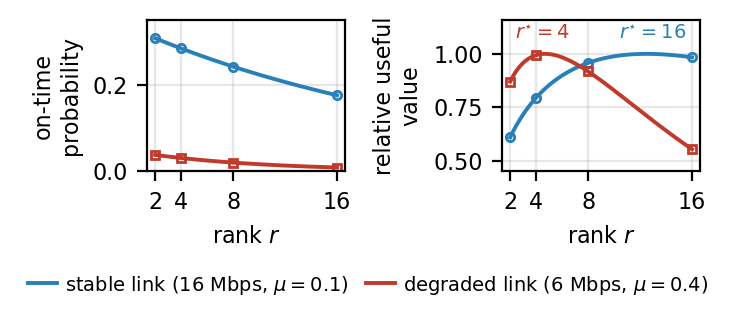
\includegraphics[width=\columnwidth]{fig_tradeoff.png}
\caption{Rank as a scheduling variable ($\tau{=}0.25$\,s, $s(r){=}0.02r{+}0.5$): a degraded link collapses the on-time probability and moves the useful-value peak from rank 16 to 4 (right panel normalized).}
\label{fig:tradeoff}
\end{figure}

\subsection{Exact dynamic program}
\label{sec:solver}
Problem \eqref{eq:objective}--\eqref{eq:constraints} with $\hat P$ in place of $P$ is a multiple-choice knapsack with an additional cardinality constraint. With the budget discretized into steps $\delta{=}0.05$\,MB, let $V_i(k,e)$ be the maximum expected useful-update value from the first $i$ clients using $k$ admissions and $e{=}\lceil B/\delta\rceil$ grid units, and let $u_i(r)=G_i^t(r)\hat P_{{\rm on},i}^t(r)$; $V_0(0,0)=0$ and all other states are $-\infty$:
\begin{equation}
\begin{aligned}
V_i(k,e)=\max\Big\{&V_{i-1}(k,e),\\
&\max_{r\in\mathcal R}\big[V_{i-1}(k{-}1,\,e{-}\lceil B_i^t(r)/\delta\rceil){+}u_i(r)\big]\Big\},
\end{aligned}
\label{eq:dp}
\end{equation}
with backpointers recovering the assignment.

\begin{proposition}[Per-round optimality]
\label{prop:opt}
Recurrence \eqref{eq:dp} yields the exact optimum of the estimated per-round problem \eqref{eq:objective}--\eqref{eq:constraints} on the discretized budget grid: $V^*_{|\mathcal D|}=\max_{k\le K,\,e\le B_{\max}/\delta}V_{|\mathcal D|}(k,e)$, with backpointers, is globally optimal.
\end{proposition}
\begin{proof}
Admitting client $i$ at rank $r$ consumes one admission slot and $\lceil B_i^t(r)/\delta\rceil$ grid units and adds $u_i(r)$, independent of other clients' choices, so $(k,e)$ summarizes all interaction and the standard interchange argument for multiple-choice knapsack applies by induction on $i$.
\end{proof}

The complexity is $O(|\mathcal D|\,K\,(B_{\max}/\delta)\,|\mathcal R|)$ time on a grid of $B_{\max}/\delta$ steps and $O(K\,B_{\max}/\delta)$ memory with rolling arrays; the 0.05\,MB grid step yields runtimes of 33--836\,ms for 500 clients, linear up to 1000 clients (Section~\ref{sec:eval}). Algorithm~\ref{alg:scheduler} summarizes the round.

\begin{algorithm}[t]
\caption{Deadline-aware adaptive-rank scheduling for one round}
\label{alg:scheduler}
\footnotesize
\begin{algorithmic}[1]
\REQUIRE $\mathcal D$, $\mathcal R$, $K$, $B_{\max}$, $\tau$, $\{x_i^t\}$, and $\delta$
\ENSURE Client--rank assignment and timely aggregation
\STATE Estimate $\hat P_{\mathrm{on},i}^t(r)$ using \eqref{eq:hazard} and compute $G_i^t(r)$ using \eqref{eq:cap} for all $i\in\mathcal D$ and $r\in\mathcal R$
\STATE Set $V_0(0,0)=0$ and all other states to $-\infty$
\FOR{$i=1,\ldots,|\mathcal D|$, $k=0,\ldots,K$, $e=0,\ldots,\lfloor B_{\max}/\delta\rfloor$}
    \STATE Set $V_i(k,e)\leftarrow V_{i-1}(k,e)$
    \FOR{each $r\in\mathcal R$ with $q_i(r)=\lceil B_i^t(r)/\delta\rceil\leq e$ and $k\geq1$}
        \STATE $u_i(r)\leftarrow G_i^t(r)\hat P_{\mathrm{on},i}^t(r)$
        \STATE $V_i(k,e)\leftarrow\max\{V_i(k,e),V_{i-1}(k-1,e-q_i(r))+u_i(r)\}$; store backpointer
    \ENDFOR
\ENDFOR
\STATE Select $(k^\star,e^\star)=\arg\max_{0\leq k\leq K,\,0\leq e\leq\lfloor B_{\max}/\delta\rfloor}V_{|\mathcal D|}(k,e)$
\STATE Backtrack from $(k^\star,e^\star)$ to recover the client--rank assignment
\STATE Execute assignments and collect updates received before $\tau$
\STATE Aggregate timely updates by rank-masked averaging over the frozen factor
\STATE Update link-state history and mobility features for the next round
\end{algorithmic}
\end{algorithm}

\subsection{Rank-masked aggregation with frozen factors}
\label{sec:aggregation}
Two details make heterogeneous-rank aggregation sound in the shared $r_{\max}$ coordinate system. \emph{Factor masking}: a rank-$r$ update activates only the first $r$ rows of $A$ and columns of $B$; averaging normalizes each coordinate by the weight of clients activating it, preventing low-rank updates from diluting high-rank coordinates \cite{wang2024flora,babakniya2023slora}. \emph{Frozen factors}: we freeze $A$ at the shared server-side initialization and train only $B$ locally, inheriting the frozen-factor device from FFA-LoRA \cite{sun2024ffalora}; the novelty is the scheduling context. Because every client optimizes in the same $A$-induced coordinates, averaging $B$ is exactly averaging the induced update $\Delta W$---whereas jointly trained $(A,B)$ pairs are identifiable only up to invertible transforms, so separately averaged factors need not average the updates at all. 

\section{Performance Evaluation}
\label{sec:eval}

\subsection{Setup}
\textbf{Real trainer.} A PyTorch federated LoRA trainer runs on one A800 GPU. The backbone is a 6-convolution BatchNorm CNN with two 256-wide linear layers, centrally pretrained with standard augmentation and cosine decay (30/45/3 epochs on CIFAR-10/CIFAR-100/MNIST), then frozen; LoRA adapters ($r_{\max}{=}16$, rank set $\mathcal R{=}\{2,4,8,16\}$) are placed on \emph{all six convolutions via $1{\times}1$ factors and both head layers}, so the rank genuinely bounds the capacity of every adapted weight. Backbone test accuracy is 0.914/0.692/0.995. Federated training uses 20 clients with Dirichlet($\alpha{=}0.5$) partitions, 10 participants per round, 40 rounds, five seeds (0--4); local SGD (lr $0.005$, cosine decay, gradient clipping) trains frozen-$A$ factors; the server applies rank-masked weighted averaging with momentum 0.3. Link traces follow Section~\ref{sec:model}: rate $\sim$LogNormal(2.5,\,0.7) clipped to [1,\,40]\,Mbps, mobility $\sim$Beta(2,\,5), common random numbers across methods within each seed; payload $s(r){=}0.02r{+}0.5$ normalized MB; full-parameter updates are represented at rank-64 payload (1.78\,MB)---a communication-volume alignment, not an architectural equivalence.
\textbf{Scope of the two tiers.} The trainer evaluates both the fair-cohort rank rule and the joint client--rank DP arm (10\,MB budget, cap 10); the simulator extends the joint scheduler to 500 clients, where participation is part of the decision.
\textbf{Simulator.} A 500-client, 150-round scheduler simulation applies the same delivery and capacity models end-to-end in the fair-cohort variant with the saturating proxy $acc_{t+1}=\mathrm{clip}(acc_t+0.08\,\mathrm{gain}_t(1-acc_t)-0.0005\,acc_t+\varepsilon,\,0,1)$, $acc_0{=}0.1$, over nine regimes: nominal; deadlines \{0.25, 0.5, 2.0\}\,s; budgets \{12, 40\}\,MB; mobility stress; and a 1000-client scenario; five seeds with common traces.
\textbf{Solver study.} 30 instances per (deadline, budget) cell at 500 clients compare the exact DP with value-per-byte greedy---value greedy and fixed rank 16 track it within 6.1\% and are omitted from Table~\ref{tab:dp} (reproducibility artifact)---plus a 1000-client sweep.

\begin{table}[t]
\centering
\caption{Real trainer, non-IID CIFAR-10 (five seeds): nominal deadline and 0.25\,s stress. DP-joint schedules all 20 clients under a 10\,MB budget (cap 10); the other arms sample 10 uniformly. Accuracy at round 40 (mean$\pm$std); timely ratio, bytes/round, and delivered mean rank averaged over rounds 30--39.}
\label{tab:trainer}
\centering\footnotesize
\resizebox{\columnwidth}{!}{%
\begin{tabular}{l cccc cccc}
\toprule
& \multicolumn{4}{c}{Nominal deadline} & \multicolumn{4}{c}{Deadline 0.25\,s}\\
\cmidrule(lr){2-5}\cmidrule(lr){6-9}
Method & Acc. & Timely & Bytes & Rank & Acc. & Timely & Bytes & Rank\\
\midrule
FedAvg (full) & $0.9138{\pm}.0019$ & 0.28 & 17.8 & 64 & $0.9137{\pm}.0026$ & 0.04 & 17.8 & 64\\
FedLoRA $r{=}4$ & $0.9145{\pm}.0012$ & 0.50 & 5.8 & 4 & $0.9147{\pm}.0019$ & 0.21 & 5.8 & 4\\
FedLoRA $r{=}16$ & $0.9142{\pm}.0016$ & 0.44 & 8.2 & 16 & $0.9142{\pm}.0019$ & 0.15 & 8.2 & 16\\
Random rank & $0.9144{\pm}.0016$ & 0.49 & 6.5 & 7.4 & $0.9148{\pm}.0017$ & 0.17 & 6.5 & 6.5\\
Adaptive (fair-cohort) & $0.9143{\pm}.0015$ & 0.44 & 8.1 & 16.0 & $0.9145{\pm}.0020$ & 0.16 & 7.1 & 13.5\\
DP-joint (ours) & $0.9140{\pm}.0006$ & 0.57 & 7.9 & 14.7 & $0.9142{\pm}.0012$ & 0.22 & 7.6 & 12.9\\
\bottomrule
\end{tabular}%
}
\end{table}

\begin{table}[t]
\centering
\caption{Federated accuracy on CIFAR-100 and MNIST (five seeds, round 40, mean$\pm$std). Network metrics are dataset-invariant by construction (shared traces); the 0.25\,s stress timely ratios match Table~\ref{tab:trainer}.}
\label{tab:datasets}
\centering\footnotesize
\resizebox{\columnwidth}{!}{%
\begin{tabular}{l cccc}
\toprule
& \multicolumn{2}{c}{CIFAR-100} & \multicolumn{2}{c}{MNIST}\\
\cmidrule(lr){2-3}\cmidrule(lr){4-5}
Method & Nominal & 0.25\,s & Nominal & 0.25\,s\\
\midrule
FedAvg (full) & $0.6926{\pm}.0023$ & $0.6924{\pm}.0021$ & $0.9945{\pm}.0015$ & $0.9946{\pm}.0009$\\
FedLoRA $r{=}4$ & $0.6927{\pm}.0019$ & $0.6928{\pm}.0022$ & $0.9948{\pm}.0006$ & $0.9948{\pm}.0006$\\
FedLoRA $r{=}16$ & $0.6929{\pm}.0020$ & $0.6927{\pm}.0017$ & $0.9950{\pm}.0007$ & $0.9949{\pm}.0006$\\
Random rank & $0.6929{\pm}.0022$ & $0.6928{\pm}.0020$ & $0.9949{\pm}.0006$ & $0.9949{\pm}.0007$\\
Adaptive (fair-cohort) & $0.6928{\pm}.0020$ & $0.6925{\pm}.0020$ & $0.9950{\pm}.0007$ & $0.9949{\pm}.0006$\\
\bottomrule
\end{tabular}%
}
\end{table}

\begin{figure}[t]
\centering
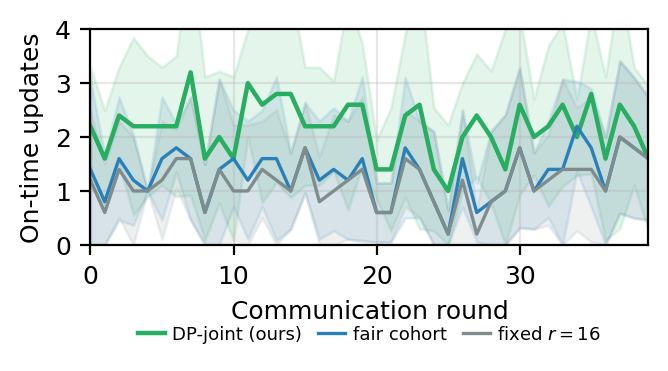
\includegraphics[width=\columnwidth]{fig_dp_timely.png}
\caption{On-time updates per round in the real trainer under the 0.25\,s deadline (mean$\pm$std, five seeds): the joint client--rank DP arm sustains more on-time updates than the fair cohort and fixed rank 16.}
\label{fig:dp_timely}
\end{figure}

\begin{figure}[t]
\centering
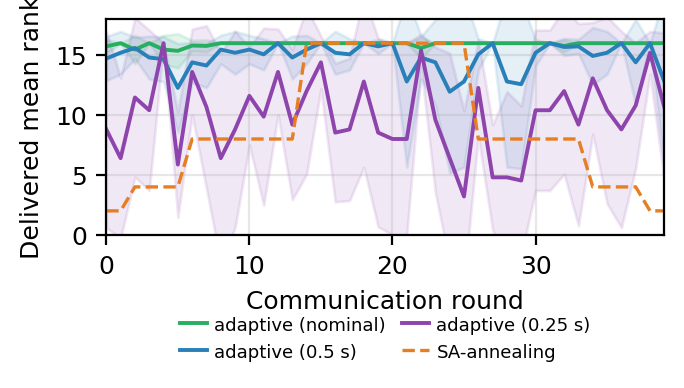
\includegraphics[width=\columnwidth]{fig_rank_dynamics.png}
\caption{Delivered mean rank per round: the adaptive rule tracks deadline pressure ($\tau{=}1$/$0.5$/$0.25$\,s; mean over five seeds), while the link-oblivious annealed schedule sweeps blindly.}
\label{fig:rank_dyn}
\end{figure}

\subsection{Impact of rank on accuracy and traffic}

Table~\ref{tab:trainer} reports five-seed means$\pm$std after 40 rounds. Fixed $r{=}4$, fixed $r{=}16$, random, and adaptive LoRA remain within one standard deviation of the backbone accuracy. Volume-aligned full-parameter updates achieve similar accuracy but spend 17.8 normalized MB per round versus 5.8--8.2 for LoRA ($2.2$--$3.1\times$ more) and deliver a smaller fraction on time (0.28 vs 0.44--0.50). Accuracy trajectories remain stable over all 40 rounds and across datasets; Table~\ref{tab:datasets} reports the federated CIFAR-100 and MNIST runs. The joint client--rank DP arm (all 20 clients under a 10\,MB budget) reaches the same accuracy with a higher on-time fraction (0.57 vs 0.44) at fewer bytes (Fig.~\ref{fig:dp_timely}).

\subsection{Adaptive ranking under deadline stress}
Under the 0.25\,s deadline (Table~\ref{tab:trainer}, right), the fair-cohort adaptive rule downshifts. Its delivered mean rank falls from 16.0 (nominal) to 15.5 at 0.5\,s and 13.5 at 0.25\,s (Fig.~\ref{fig:rank_dyn})---exactly the regime where the delivery hazard \eqref{eq:hazard} makes rank-16 payloads marginal---while the loose-deadline control (2\,s) restores rank 16.0. Downshifting pays: adaptive matches fixed $r{=}16$ accuracy (0.9145 vs 0.9142) while transmitting 14\% fewer bytes (five-seed means 7.07 vs 8.20\,MB) and delivering a comparable number of updates per round. Full-parameter updates collapse: their timely ratio falls from 0.28 (nominal, Table~\ref{tab:trainer}) to 0.13 at 0.5\,s and 0.04 at 0.25\,s, at unchanged $2.2\times$ bytes. A mobility-only scenario leaves adaptive at the top rank; extreme heterogeneity ($\alpha{=}0.1$) costs rank-16 about 0.3 points relative to rank 4; repeating the 0.25\,s stress on CIFAR-100 and MNIST reproduces the CIFAR-10 picture (Table~\ref{tab:datasets}). The DP-joint arm sustains 0.22 vs 0.16 on-time updates for the fair cohort at 7.56\,MB; every seed pair favors it, a directional result at five seeds ($p{=}0.062$, the smallest attainable).

\subsection{External baselines and ablations}
Three external baselines are added to the prototype (five seeds): an SA-FedLoRA-style schedule annealing the rank from 2 to 16 over the 40 rounds, oblivious to link state \cite{yang2024safedlora}; an Oort-style top-$K$-of-$2K$ selector by data-size-and-recency utility at fixed rank \cite{oort2021oort}; and joint $A/B$ training with plain averaging \cite{guo2025fedsalora}---all within noise of the backbone, as parity predicts. Under the 0.25\,s deadline the annealed schedule sits at low rank by construction and delivers the most updates per round (2.0 vs 1.6) at the fewest bytes, but cannot upshift (Fig.~\ref{fig:rank_dyn}); in the simulator it settles at rank 2, losing 8.2 points of scheduling accuracy to the network-aware rule nominally and 3.9 under stress. The Oort-style selector cannot trade capacity against delivery at fixed rank. Component ablations show no removal changes final accuracy in the parity regime; instead they shape network behavior: removing the capacity term collapses the rule to rank 2 (bytes 5.40, delivered rank 2.0)---whose capacity cost is material in the simulator; at elevated lr ($0.02$), joint $A/B$ training shows a markedly deeper transient accuracy dip (minimum 0.901 vs 0.909), matching the factor-rotation analysis of Section~\ref{sec:aggregation}. Sensitivity sweeps over the provisioned width ($r_{\max}$ 8$\to$32: bytes 6.6$\to$10.6, accuracy flat), heterogeneity ($\alpha$ 0.1$\to$1.0: accuracy 0.911$\to$0.915), and cohort size ($K$ 5$\to$20: delivered updates 2.3$\to$8.6, accuracy flat) confirm $r_{\max}$ and $K$ are provisioning knobs, not accuracy knobs; the rank rule costs 105\,$\mu$s per client--rank decision.

\subsection{Scheduling at 500-client scale}
Table~\ref{tab:sim} summarizes the simulator. In the nominal regime, adaptive matches the best fixed rank (0.778) at slightly fewer bytes, and both clearly outperform random rank, rank 4, and full updates. Under stress the separation grows: at 0.25\,s, adaptive reaches 0.413 versus 0.404 for fixed $r{=}16$, 0.359 for random, and 0.187 for full updates (timely 0.037). Under the binding 12\,MB budget adaptive and $r{=}16$ tie at 0.687---the cap, not the rank, binds; in the mobility-stress and 1000-client regimes adaptive again matches or exceeds the best fixed rank; across all nine regimes it matches the best method to within 0.001 (Fig.~\ref{fig:sim}).

\begin{table}[t]
\centering
\caption{Scheduler simulation, 500 clients, 150 rounds (five seeds, final round). Accuracy is the bounded scheduling proxy; bytes are per-round totals.}
\label{tab:sim}
\centering\footnotesize
\resizebox{\columnwidth}{!}{%
\begin{tabular}{l ccc ccc cc}
\toprule
& \multicolumn{3}{c}{Nominal} & \multicolumn{3}{c}{Deadline 0.25\,s} & \multicolumn{2}{c}{12\,MB budget / 1000 clients}\\
\cmidrule(lr){2-4}\cmidrule(lr){5-7}\cmidrule(lr){8-9}
Method & Proxy & Timely & Bytes & Proxy & Timely & Bytes & 12\,MB & 1000\\
\midrule
FedAvg & 0.607 & 0.26 & 44.5 & 0.187 & 0.04 & 44.5 & 0.397 & 0.577\\
$r{=}4$ & 0.606 & 0.51 & 14.5 & 0.343 & 0.20 & 14.5 & 0.576 & 0.610\\
$r{=}16$ & \textbf{0.778} & 0.44 & 20.5 & 0.404 & 0.14 & 20.5 & \textbf{0.687} & \textbf{0.781}\\
Random & 0.666 & 0.48 & 16.5 & 0.359 & 0.18 & 16.5 & 0.620 & 0.668\\
SA-annealing & 0.696 & 0.52 & 13.5 & 0.374 & 0.22 & 13.5 & 0.636 & 0.699\\
Reliability-only & 0.508 & 0.52 & 13.5 & 0.292 & 0.22 & 13.5 & 0.493 & 0.511\\
Adaptive (ours) & \textbf{0.778} & 0.44 & 20.3 & \textbf{0.413} & 0.15 & 17.8 & \textbf{0.687} & \textbf{0.781}\\
\bottomrule
\end{tabular}%
}
\end{table}

\begin{figure}[t]
\centering
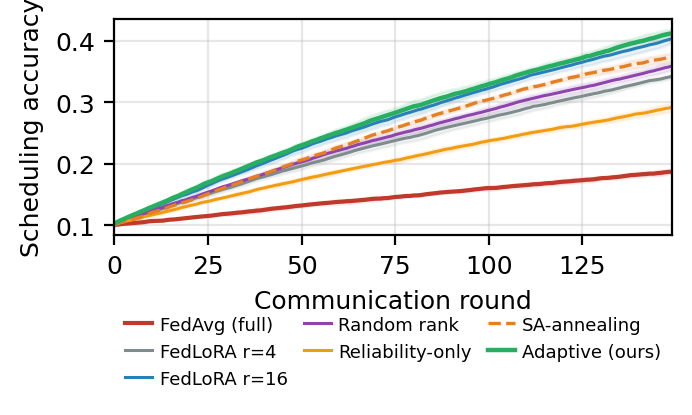
\includegraphics[width=\columnwidth]{fig_sim_stress.png}
\caption{Scheduler simulation under the 0.25\,s deadline (bounded scheduling proxy; mean$\pm$std, five seeds): adaptive downshifting separates from fixed rank 16 and outperforms random, reliability-only, SA-annealing, and full updates.}
\label{fig:sim}
\end{figure}

\subsection{Optimality gap and runtime}
\label{sec:dp_study}
Table~\ref{tab:dp} reports the solver study: greedy heuristics are near-optimal when the budget is slack but lose 4.5--6.1\% when it binds (12\,MB), and up to 10\% under a tight deadline even with slack budget, because per-byte ordering misprices delivery risk. The exact DP attains the discretized optimum in every cell; runtime is 33--836\,ms for 500 clients (dominated by the grid size), scaling linearly to 1000 clients---means over 30 instances, single-threaded NumPy on an Intel Xeon Platinum 8358, timing the recurrence only. A grid sweep over 0.2--0.01\,MB steps shows the objective is step-insensitive when the budget is slack; at the binding 12\,MB budget the 0.05\,MB default deviates at most 3.1\% from a 0.01\,MB reference, and a 0.025\,MB step bounds the deviation by 1.3\% at $\sim$1.7$\times$ runtime. The fair-cohort variant used by the trainer reaches 27--55\% of the unconstrained DP objective.

\begin{table}[t]
\centering
\caption{Solver study (500 clients, $K{=}25$, 30 instances per cell): optimality gap of value-per-byte greedy relative to the exact DP, and DP runtime.}
\label{tab:dp}
\centering\footnotesize
\begin{tabular}{cc c c}
\toprule
Deadline (s) & Budget (MB) & Greedy val/byte gap & DP time (ms)\\
\midrule
1.0  & 300 & 0.0\% & 836\\
1.0  & 40  & 0.0\% & 92\\
1.0  & 12  & 6.1\% & 33\\
0.5  & 300 & 0.7\% & 833\\
0.5  & 40  & 0.8\% & 92\\
0.5  & 12  & 5.6\% & 33\\
0.25 & 300 & 9.7\% & 830\\
0.25 & 40  & \textbf{10.0\%} & 92\\
0.25 & 12  & 4.5\% & 33\\
\bottomrule
\end{tabular}
\end{table}

\section{Discussion and Limitations}
\label{sec:discussion}
\textbf{Scope.} The trainer demonstrates parity, not rank-dependent accuracy gains; claims that low rank limits adaptation quality would require longer horizons, weaker backbones, or shifted clients, and the simulator's capacity model is a scheduling abstraction. Neglected fixed delays reduce the effective deadline equally for all ranks---rank ordering is largely preserved while absolute timely ratios are overestimated. $\bar R_i^t$ is each client's effective rate under current cell load; uploads are parallel, so the budget is a payload-level proxy rather than an airtime reservation---an explicit shared-bandwidth model is future work. \textbf{Backbone pretraining.} Centralized pretraining follows parameter-efficient FL practice; without a server-side corpus it would need self-supervised or public data, and parity should be re-verified. \textbf{Generality.} The prototype validates CNN adapters at $r_{\max}{=}16$ with synthetic traces; transformer backbones and measured links change constants, not the formulation. \textbf{Estimator and myopia.} The hazard form \eqref{eq:hazard} assumes exponential realizations and should be calibrated per client from observed outcomes (a plug-in for the scheduler). A robustness check with lognormal rate-estimation error ($\sigma{=}0.2$) degrades the objective by $\le$5.1\% on average (9.4\% worst case) in the binding regime, and linear or logarithmic gain shapes change admission for $\le$0.5\% of clients; the DP remains exact for the estimated per-round problem, not the multi-round control problem induced by budget carry-over and mobility correlation. \textbf{Security.} Formal privacy guarantees require differential privacy or secure aggregation, which compose orthogonally with rank scheduling \cite{bonawitz2017secureagg,wei2023pfl_dp}.

\section{Conclusion}
\label{sec:conclusion}
This paper formulated Federated LoRA over mobile edge networks as deadline-aware client--rank scheduling. A rank-dependent delivery model connects adapter size to timeliness, and a pseudo-polynomial dynamic program optimally solves the budget-discretized, estimated per-round assignment. Frozen-factor rank-masked averaging supports heterogeneous client ranks. A 10-seed replication (the five-seed tables plus seeds 5--9; paired two-sided Wilcoxon, $n{=}10$) confirms the network-side differences at the 0.05 level: under the evaluated pretrained-CNN settings, adaptive ranking saves 14\% of update bytes against fixed rank 16 (means 7.01 vs 8.20\,MB, $p{=}0.002$) and delivers more on-time updates ($p{=}0.016$), with no significant accuracy difference ($p{=}0.40$); volume-aligned full-parameter updates use $2.2\times$ the bytes and deliver only 4\% of scheduled updates on time at 0.25\,s. The dynamic program improves expected useful updates by up to 10\% over greedy scheduling in binding regimes at sub-second cost.

\section*{Acknowledgment}
This work was supported by the project Research on Advanced Threat Awareness Technology Based on Dynamic Execution Behavior Adjudication in Cloud Environments (FFX24641X028). The authors also thank the Information Engineering University research group for discussions and experimental assistance.

\bibliographystyle{IEEEtran}
\bibliography{references}

\end{document}
